\chapter{Scenarii de utilizare}
\label{chapter:scenariiUtilizare}


\section{Înregistrare si autentificare utilizator}
\label{sec:inregistrare-utilizator}


Înregistrarea și autentificarea utilizatorilor se face după un proces clasic, în care dacă utilizatorul există deja,
se va autentifica cu numele de utilizator și parola, iar dacă nu există, se va înregistra cu un email și o parolă.
În caz de succes la înregistrare se trimit datele în back-end, se stocheaza în baza de date, se va afișa un mesaj de succes
și se va porni animatația de succes la înregistrare a mascotei balon. După înregistrare, utilizatorul poate intra în 
pagina de logare și se poate autentifica cu datele introduse la înregistrare. Înregistrarea are două moduri posibile
pentru conturi de profesor și conturi de elev.

În cazul în care utilizatorul nu există, se va afișa un mesaj de eroare și se va rămâne pe pagina de logare.
În cazul în care utilizatorul credentțialele sunt corecte și există în sistem se va afișa un mesaj de succes,
se va face animatia mascotei balon pentru logare și se va redirecționa utilizatorul către pagina principală a aplicației.
Modelul 3D al mascotei este responsiv și la scrierea caraterelor în promptul de înregistrare și logare.


\begin{figure}[htb]
  \centering
  \subfloat[Înregistrare utilizator\label{fig:register}]{
    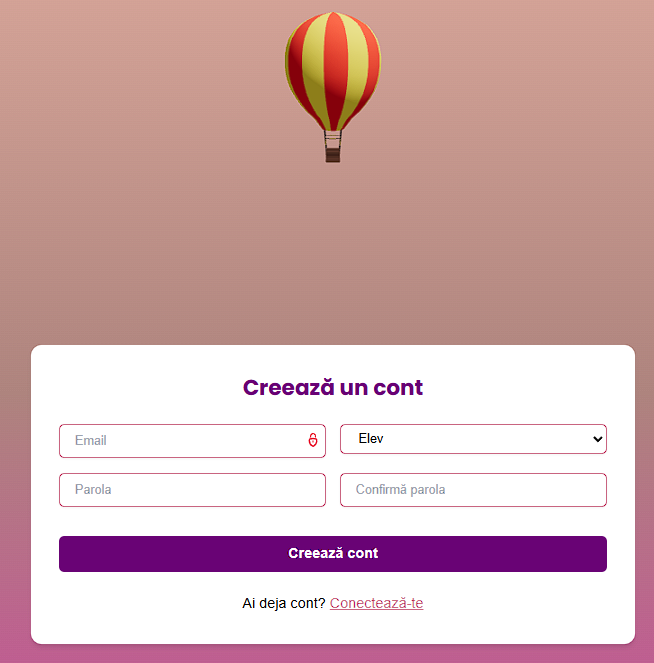
\includegraphics[width=0.53\textwidth]{imgs/register.png}
  }
  \hfill
  \subfloat[Autentificare utilizator\label{fig:login}]{
    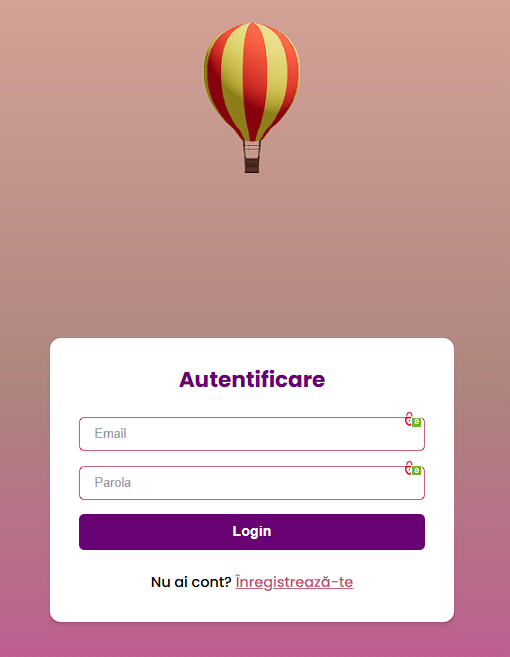
\includegraphics[width=0.42\textwidth]{imgs/login.png}
  }
  \caption{Înregistrare și autentificare utilizator}
  \label{fig:portainer-sidebyside}
\end{figure}

\newpage
\section{Explorarea meniul principal}
\label{sec:explorare-meniu-principal}

Meniul principal al aplicației este afișat după autentificare și conține un model 3D principal cu on insulă mare și mai multe insule
mici care reprezintă secțiunile educaționale disponibile în aplicație. Navigarea se face prin rotire cu mouse-ul. Restul meniului 
este reprezentat print-o bară clasică de navigare în partea de sus a ecranului, care conține butoane pentru accesarea profilului,
magazinului de cărți, secțiunilor despre și contact.

\fig[width=0.9\textwidth]{imgs/mainmenu.png}{fig:interfata}{Interfața meniului principal}


\begin{figure}[htb]
  \centering
  \subfloat[Magazinul online\label{fig:magazin}]{
    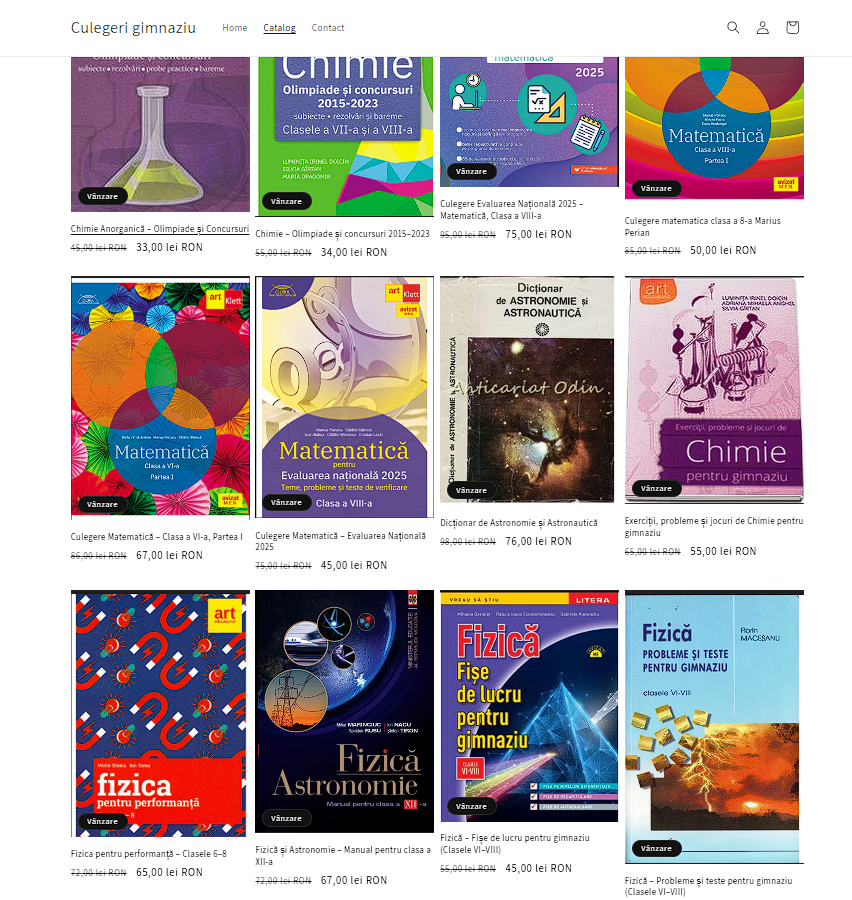
\includegraphics[width=0.55\textwidth]{imgs/magazin.png}
  }
  \hfill
  \subfloat[Pagina de contact\label{fig:contact}]{
    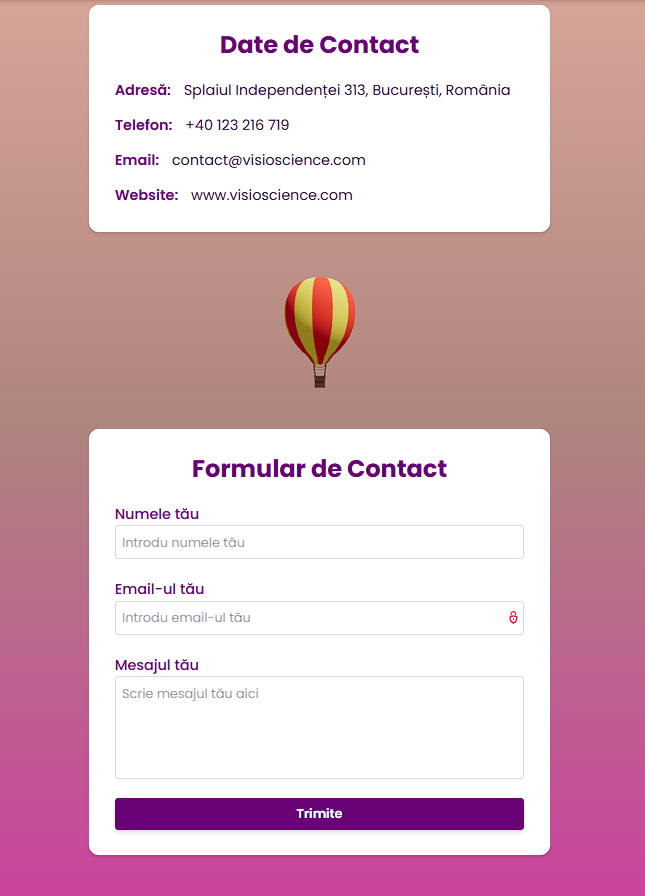
\includegraphics[width=0.4\textwidth]{imgs/contact.png}
  }
  \caption{Magazinul online și pagina de contact}
  \label{fig:portainer-sidebyside}
\end{figure}


\section{Accesarea secțiunilor educaționale}
\label{subsec:accesare-sectiuni-educationale}

Fiecare secțiune conține multiple scene 3D educaționale care reprezintă noțiuni sau fenomene specifice domeniului respectiv.
Cu fiecare dintre ele se poate interacționa prin rotirea camerei, zoom și mișcarea camerei în jurul scenei.
Pentru secțiunea de geometrie avem următoarele scene 3D educaționale:
\begin{itemize}
    \item \textbf{Cub}
    \item \textbf{Piramidă}
    \item \textbf{Paralelipiped}
    \item \textbf{Cilindru}
    \item \textbf{Con}
    \item \textbf{Sferă}
\end{itemize}

\fig[width=1\textwidth]{imgs/mathex.png}{fig:explorare-mathematica}{Exemplu de scenă de matematică}

\newpage
Pentru materia de fizică avem următoarele scene 3D educaționale:

\begin{itemize}
    \item \textbf{Plan înclinat}
    \item \textbf{Scripete simplu}
    \item \textbf{Scripete mobil}
    \item \textbf{Pendul și oscilații}
    \item \textbf{Resort și legea lui Hooke}
    \item \textbf{Mișcarea circulară uniformă}
    \item \textbf{Mișcarea de proiectil}
    \item \textbf{Cădere liberă}
    \item \textbf{Coliziune elastică}
    \item \textbf{Coliziune plastică}
\end{itemize}

\fig[width=1\textwidth]{imgs/fizicaex.png}{fig:explorare-fizica}{Exemplu de scenă de fizică}


\newpage
Pentru materia de chimie avem scene educaționale customizabile prin încărcarea manuală a moleculelor chimice în format .mol, ele fiind
parsate și transmise înapoi la front-end care le transformă în scene 3D.

\fig[width=1\textwidth]{imgs/chimieex.png}{fig:explorare-chimie}{Exemplu de scenă de chimie}

În cazul scenelor de astronomie avem suport pentru toate planetaele din sistemul solar, cât și pentru sistemul solar în sine cu 
animația rotațiilor planetelor.

\fig[width=1\textwidth]{imgs/astronomieex.png}{fig:explorare-astronomie}{Exemplu de scenă de astronomie}


\newpage
Și ultima materie suportată curent este informatica care conține scene educaționale despre structuri de date și algoritmi,
cum ar fi:

\begin{itemize}
    \item \textbf{Array}
    \item \textbf{Vector}
    \item \textbf{Unordered Map}
    \item \textbf{Ordered Map}
    \item \textbf{Unordered Set}
    \item \textbf{Ordered Set}
    \item \textbf{Multiset}
    \item \textbf{PriorityQueue}
    \item \textbf{Deque}
    \item \textbf{Stack}
    \item \textbf{Queue}
    \item \textbf{List}
    \item \textbf{Doubly Linked List}
\end{itemize}
\fig[width=1\textwidth]{imgs/infoex.png}{fig:explorare-informatica}{Exemplu de scenă de informatică}

\section{Interacțiunea cu scenele 3D educaționale}
\label{subsec:interactiune-scene-3d}

Pe lângă interacțiunea clasică cu scenele 3D prin rotirea camerei, zoom și mișcare, la secțiunea de chimie se pot defini propriile
molecule chimice prin fișiere cu format .mol. Alt tip de interacțiune este de exemplu prin operațiile de modificare a structurilor de date
și algoritmilor din secțiunea de informatică, unde se pot adăuga sau elimina elemente din structuri de date, se pot vizualiza
elementele și se pot anima operațiile de inserare, ștergere sau căutare a elementelor în structuri de date.

\begin{figure}[htb]
  \centering
  \subfloat[Formular de încărcare molecule\label{fig:molform}]{
    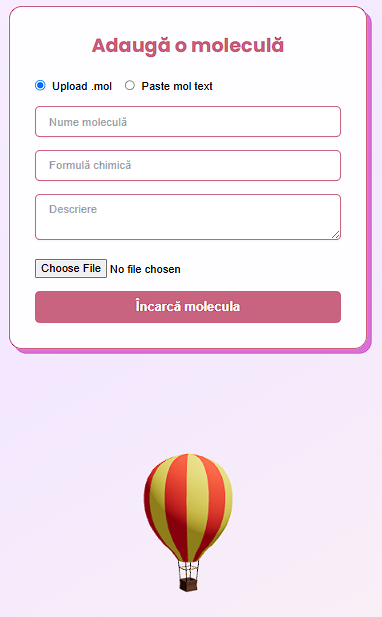
\includegraphics[width=0.25\textwidth]{imgs/molform.png}
  }
  \hfill
  \subfloat[Operații pe structuri de date\label{fig:infoops}]{
    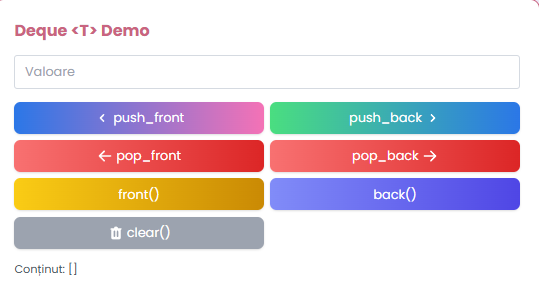
\includegraphics[width=0.55\textwidth]{imgs/infoops.png}
  }
  \caption{Interacțiunea cu scenele 3D educaționale}
  \label{fig:portainer-sidebyside}
\end{figure}

\section{Gestionarea profilului de profesor}
\label{sec:gestionare-profil-utilizator}

\subsection{Crearea de clase și gestionarea elevilor}
\label{subsec:creare-clase-elevi}

\subsection{Crearea de teste și gestionarea lor}
\label{subsec:creare-teste}

\subsection{Vizualizarea rezultatelor}
\label{subsec:vizualizare-rezultate}

\section{Gestionarea contului de elev}
\label{subsec:gestionare-cont-elev}

\subsection{Intrarea în clasele profesorului}
\label{subsec:intrare-clase-profesor}

\subsection{Accesarea testelor și vizualizarea rezultatelor}
\label{subsec:accesare-teste-elev}

\subsection{Rezolvarea testelor}
\label{subsec:rezolvare-teste}